\begin{frame}[fragile]\frametitle{Starting Point: Familiar Equations}
  \begin{itemize}
    \item Consider the system from 10th class
    \item $2x + 3y = 6$ and $x - y = 3$
    \item Multiply second by 2: $2x - 2y = 6$
    \item Subtract from first: $5y = 0 \Rightarrow y = 0$
    \item Substitute back: $x = 3$
    \item Solution: $(3, 0)$ — unique answer
  \end{itemize}
\end{frame}

\begin{frame}[fragile]\frametitle{Three Types of Solutions}
  \begin{itemize}
    \item \textbf{Unique solution}: One intersection point
    \item Example: $2x + 3y = 6$, $x - y = 3 \Rightarrow (3,0)$
    \item \textbf{No solution}: Parallel lines never meet
    \item Example: $x + 2y = 6$, $2x + 4y = 8$
    \item \textbf{Infinite solutions}: Coincident lines overlap
    \item Example: $x + 2y = 6$, $2x + 4y = 12$
    \item Key insight: 0, 1, or $\infty$ solutions (never 2, 3, or 4)
  \end{itemize}
\end{frame}

\begin{frame}[fragile]\frametitle{Graphical Method: Unique Solution}
  \begin{columns}
    \begin{column}[T]{0.6\linewidth}
      \begin{itemize}
        \item Plot both equations as lines
        \item $2x + 3y = 6$ (blue line)
        \item $x - y = 3$ (red line)
        \item Lines intersect at exactly one point
        \item Intersection = unique solution $(3, 0)$
        \item One intersection $\Rightarrow$ unique answer
      \end{itemize}
    \end{column}
    \begin{column}[T]{0.4\linewidth}
      \begin{center}
        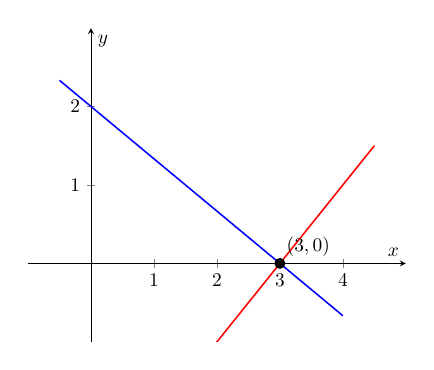
\begin{tikzpicture}[scale=0.7]
          \begin{axis}[
            axis lines=center,
            xlabel=$x$, ylabel=$y$,
            xmin=-1, xmax=5, ymin=-1, ymax=3,
            xtick={0,1,2,3,4}, ytick={0,1,2}
          ]
          \addplot[blue, thick, domain=-0.5:4] {(6-2*x)/3};
          \addplot[red, thick, domain=0:4.5] {x-3};
          \node[circle,fill,inner sep=2pt] at (3,0) {};
          \node[above right] at (3,0) {$(3,0)$};
          \end{axis}
        \end{tikzpicture}
      \end{center}
    \end{column}
  \end{columns}
\end{frame}

\begin{frame}[fragile]\frametitle{Other Solution Cases}
  \begin{columns}
    \begin{column}[T]{0.6\linewidth}
      \begin{itemize}
        \item \textbf{No solution}: Parallel lines
        \item $x + 2y = 7$ and $2x + 4y = 9$
        \item Zero intersection points
        \item \textbf{Infinite solutions}: Coincident lines
        \item $x + 2y = 7$ and $2x + 4y = 14$
        \item Every point on line is a solution
      \end{itemize}
    \end{column}
    \begin{column}[T]{0.4\linewidth}
      \begin{center}
        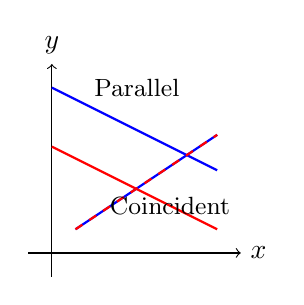
\begin{tikzpicture}[scale=0.6]
          \draw[->] (-0.5,0) -- (4,0) node[right] {$x$};
          \draw[->] (0,-0.5) -- (0,4) node[above] {$y$};
          \draw[blue, thick] (0,3.5) -- (3.5,1.75);
          \draw[red, thick] (0,2.25) -- (3.5,0.5);
          \node at (1.8,3.5) {\small Parallel};
          \draw[blue, thick] (0.5,0.5) -- (3.5,2.5);
          \draw[red, thick, dashed] (0.5,0.5) -- (3.5,2.5);
          \node at (2.5,1) {\small Coincident};
        \end{tikzpicture}
      \end{center}
    \end{column}
  \end{columns}
\end{frame}

\begin{frame}[fragile]\frametitle{Multiple Variables: Complexity Grows}
  \begin{itemize}
    \item System with 4 variables
    \item $x + 4y - 2z + 3t = 9$
    \item $2x - y - z - t = 4$
    \item $5x + 7y + z - 2t = 7$
    \item $3x - 2y - 8z + 5t = 21$
    \item More variables $\Rightarrow$ harder to predict solution type
    \item Cannot visualize 4D geometry directly
    \item Need systematic computational methods
  \end{itemize}
\end{frame}

\begin{frame}[fragile]\frametitle{Transformation Concept}
  \begin{columns}
    \begin{column}[T]{0.6\linewidth}
      \begin{itemize}
        \item Two coordinate systems: small $xy$ and capital $XY$
        \item Equations: $X = x + 2y$, $Y = 3x - y$
        \item Small $xy$ plane: unit square
        \item Capital $XY$ plane: parallelogram
        \item Square transforms into parallelogram
        \item Stretching and rotating combined
      \end{itemize}
    \end{column}
    \begin{column}[T]{0.4\linewidth}
      \begin{center}
        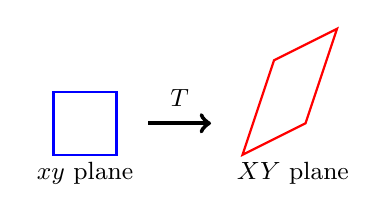
\begin{tikzpicture}[scale=0.8]
          \draw[thick, blue] (0,0) rectangle (1,1);
          \node at (0.5,-0.3) {\small $xy$ plane};
          \draw[->, ultra thick] (1.5,0.5) -- (2.5,0.5);
          \node at (2,0.9) {\small $T$};
          \draw[thick, red] (3,0) -- (4,0.5) -- (4.5,2) -- (3.5,1.5) -- cycle;
          \node at (3.8,-0.3) {\small $XY$ plane};
        \end{tikzpicture}
      \end{center}
    \end{column}
  \end{columns}
\end{frame}

\begin{frame}[fragile]\frametitle{Mathematical Spaces}
  \begin{itemize}
    \item $\mathbb{R}$: real number line (1D)
    \item $\mathbb{R}^2$: plane with two coordinates $(x, y)$
    \item $\mathbb{R}^3$: 3D space with $(x, y, z)$
    \item $\mathbb{R}^n$: n-dimensional space
    \item Dimension here means number of coordinates
    \item Not the physical space dimensions
    \item Can work with $\mathbb{R}^{100}$ mathematically
    \item Cannot visualize, but can compute
  \end{itemize}
\end{frame}

\begin{frame}[fragile]\frametitle{Notation: Real Spaces}
  \begin{itemize}
    \item Symbol $\mathbb{R}$ denotes real numbers
    \item $\mathbb{R}^2 = \{(x,y) : x,y \in \mathbb{R}\}$
    \item Column vector notation: $\begin{pmatrix} x \\ y \end{pmatrix} \in \mathbb{R}^2$
    \item Four-dimensional: $\begin{pmatrix} a \\ b \\ c \\ d \end{pmatrix} \in \mathbb{R}^4$
    \item Quantum mechanics uses $\mathbb{R}^\infty$ (infinite dimensions)
    \item Abstract mathematics handles any dimension
  \end{itemize}
\end{frame}

\begin{frame}[fragile]\frametitle{Transformation Definition}
  \begin{itemize}
    \item Transformation $T$ maps small $xy$ to capital $XY$
    \item Example: $T(x, y) = (x + 2y, 3x - y)$
    \item Input: point in $\mathbb{R}^2$, Output: point in $\mathbb{R}^2$
    \item $T: \mathbb{R}^2 \to \mathbb{R}^2$
    \item General form: $T(x,y) = (ax + by, cx + dy)$
    \item Coefficients $a, b, c, d$ define the transformation
    \item Linear transformation: powers are always 1
  \end{itemize}
\end{frame}

\begin{frame}[fragile]\frametitle{Range and Solution Space}
  \begin{itemize}
    \item \textbf{Range}: all possible outputs of $T$
    \item Given $(\alpha, \beta)$ in $XY$ plane, can we solve for $(x,y)$?
    \item Example: $(6, 4)$ belongs to range if solution exists
    \item $x + 2y = 6$ and $3x - y = 4$ has solution
    \item Therefore $(6, 4) \in \text{Range}(T)$
    \item \textbf{Solution space}: all inputs producing given output
    \item Unique solution: one input per output
    \item Infinite solutions: many inputs per output
  \end{itemize}
\end{frame}

\begin{frame}[fragile]\frametitle{Range-Solution Relationship}
  \begin{itemize}
    \item If Range = plane ($\mathbb{R}^2$) $\Rightarrow$ unique solution
    \item Every point in $XY$ maps to exactly one $(x,y)$
    \item If Range = line $\Rightarrow$ no solution or infinite solutions
    \item Only points on line have corresponding $(x,y)$
    \item If Range = point (origin) $\Rightarrow$ infinitely many solutions
    \item Trivial case: $X = 0, Y = 0$ satisfied by entire plane
    \item Pattern: range dimension determines solution type
  \end{itemize}
\end{frame}

\begin{frame}[fragile]\frametitle{Matrix Notation Introduction}
  \begin{itemize}
    \item System: $ax + by = X$ and $cx + dy = Y$
    \item Arrange coefficients in rectangular array
    \item Matrix form: $\begin{pmatrix} a & b \\ c & d \end{pmatrix}$
    \item This is a $2 \times 2$ matrix (2 rows, 2 columns)
    \item Variables: $\begin{pmatrix} x \\ y \end{pmatrix}$ (column matrix)
    \item Output: $\begin{pmatrix} X \\ Y \end{pmatrix}$
    \item Developed by Cayley around 1850s
  \end{itemize}
\end{frame}

\begin{frame}[fragile]\frametitle{Matrix Multiplication}
  \begin{columns}
    \begin{column}[T]{0.6\linewidth}
      \begin{itemize}
        \item Matrix equation: $\begin{pmatrix} a & b \\ c & d \end{pmatrix} \begin{pmatrix} x \\ y \end{pmatrix} = \begin{pmatrix} X \\ Y \end{pmatrix}$
        \item Row-column multiplication rule
        \item First row: $ax + by = X$
        \item Second row: $cx + dy = Y$
        \item Compact representation of linear system
        \item $A\mathbf{x} = \mathbf{b}$ (standard form)
      \end{itemize}
    \end{column}
    \begin{column}[T]{0.4\linewidth}
      \begin{center}
        \begin{tikzpicture}[scale=0.8]
          \node at (0,2) {$\begin{pmatrix} a & b \\ c & d \end{pmatrix}$};
          \node at (0,0.5) {$\begin{pmatrix} x \\ y \end{pmatrix}$};
          \draw[->, thick] (0.5,1.2) -- (0.5,0.8);
          \node at (2,1.2) {$=$};
          \node at (3.5,1.2) {$\begin{pmatrix} ax+by \\ cx+dy \end{pmatrix}$};
        \end{tikzpicture}
      \end{center}
    \end{column}
  \end{columns}
\end{frame}

\begin{frame}[fragile]\frametitle{Linear Transformations}
  \begin{itemize}
    \item Transformation $T$ represented by matrix $A$
    \item $T(\mathbf{x}) = A\mathbf{x}$
    \item Linear: all variables have power 1
    \item Study of linear transformations = Linear Algebra
    \item No folds, no curves (straight to straight)
    \item Composition: $U(T(\mathbf{x})) = U \cdot T \cdot \mathbf{x}$
    \item Matrix multiplication encodes transformation algebra
  \end{itemize}
\end{frame}

\begin{frame}[fragile]\frametitle{Abstract vs Geometric Mathematics}
  \begin{itemize}
    \item Two approaches to mathematics
    \item \textbf{Geometric view}: visualize diagrams, intuition
    \item Limited to 3 dimensions physically
    \item \textbf{Abstract view}: symbols, equations, no geometry
    \item Works for any dimension ($n$, even $\infty$)
    \item Einstein's relativity uses geometry
    \item Quantum mechanics requires abstract approach
    \item Both valid, abstract is more general
  \end{itemize}
\end{frame}

\begin{frame}[fragile]\frametitle{Historical Context}
  \begin{itemize}
    \item Matrix algebra developed around 1850
    \item Quantum mechanics emerged in 1925
    \item 75-year gap between theory and application
    \item Cayley had no idea QM would use this math
    \item Most successful physical theory uses linear algebra
    \item Modern applications: machine learning, AI
    \item GPT, DeepSeek, Gemini all use matrix operations
    \item Mathematical abstraction enables future physics
  \end{itemize}
\end{frame}

\begin{frame}[fragile]\frametitle{Four Methods to Study Linear Algebra}
  \begin{itemize}
    \item \textbf{Method 1}: Algebraic (elimination, substitution)
    \item Solve equations step-by-step symbolically
    \item \textbf{Method 2}: Graphical (plot lines, find intersections)
    \item Visual interpretation of solutions
    \item \textbf{Method 3}: Transformations (geometric mappings)
    \item Square to parallelogram perspective
    \item \textbf{Method 4}: Matrix notation (compact representation)
    \item Most powerful for computation and generalization
    \item Fifth method coming next lecture
  \end{itemize}
\end{frame}
